\section[AprEnDO]{AprEnDO}

A linguagem de programação utilizada é o nodejs com o framework react native para gerar aplicação em código nativo android. Para baixar os pacotes e fazer o controle dos mesmos está sendo utilizado o nvm e o yarn.

O ambiente de desenvolvimento usa um emulador para simular o jogo.

A pasta do jogo aprendo que encontra-se dentro da pasta desenvolvimento tem o projeto react-native com node.js e android, o package.json com as dependências, o index.js que é o ponto de entrada, os códigos fonte e os recursos. Também tem um arquivo makefile que por padrão abre o emulador de celular android, com permissão de superusuário inicia o servidor do react para desenvolvimento, cria no emulador a mais recente build do aplicativo e inicia o terminal para logs do celular emulador.

Os arquivos da pasta e uma breve explicação:
O arquivo index.js faz a importação dos módulos que são também as telas do jogo localizadas na pasta screen do código fonte em src. Também importa o módulo de navegação entra telas que precisa ser configurado para estar ciente das screens que antecedem a atual, sem a referência ao voltar a tela o jogo fecha. Uma configuração default que foi setada era para desaparecer a barra superior de navegação das telas, porém percebeu-se que em alguns celulares a barra aparecia e um pouco desconfigurada, já em outros modelos comportava como o esperado e estava invisível. 

A pasta android tem o código gerado pelo react-native o qual é um projeto padrão com os arquivos necessário para andoid, código fonte em .java, o arquivo manifest, gradle e arquivos de configuração. Algumas dependências do jogo em react native foram adicionadas manualmente no código nativo do android.

A pasta node\_modules apresenta os vários módulos do node instalados em \textit{background}.

A pasta resource tem as imagens de todas as equações de perguntas usada no módulo de classificação, as respostas usadas no módulo de resolução e seus arquivos index.js que mapeia o número das equações com a importação  das mesmas dentro do jogo, a importação só se da porquê todas as imagens já possuem o termo “require(‘numero da equação’)” que é pré-processada antes da escolha da equação aleatória a ser importada dentro da fase. Outro arquivo importante que tem nessa pasta é o \textbf{DADOS\_GERAIS.json} que possui os metadados das equações, quanto à todas classificações, tipo, ordem, homogeneidade e etc.

Foram desenhados processos para entender o fluxo do jogo. O primeiro processo é uma visão geral.

\begin{figure}[H]
\centering
\caption{Processo geral do jogo aprEnDO}
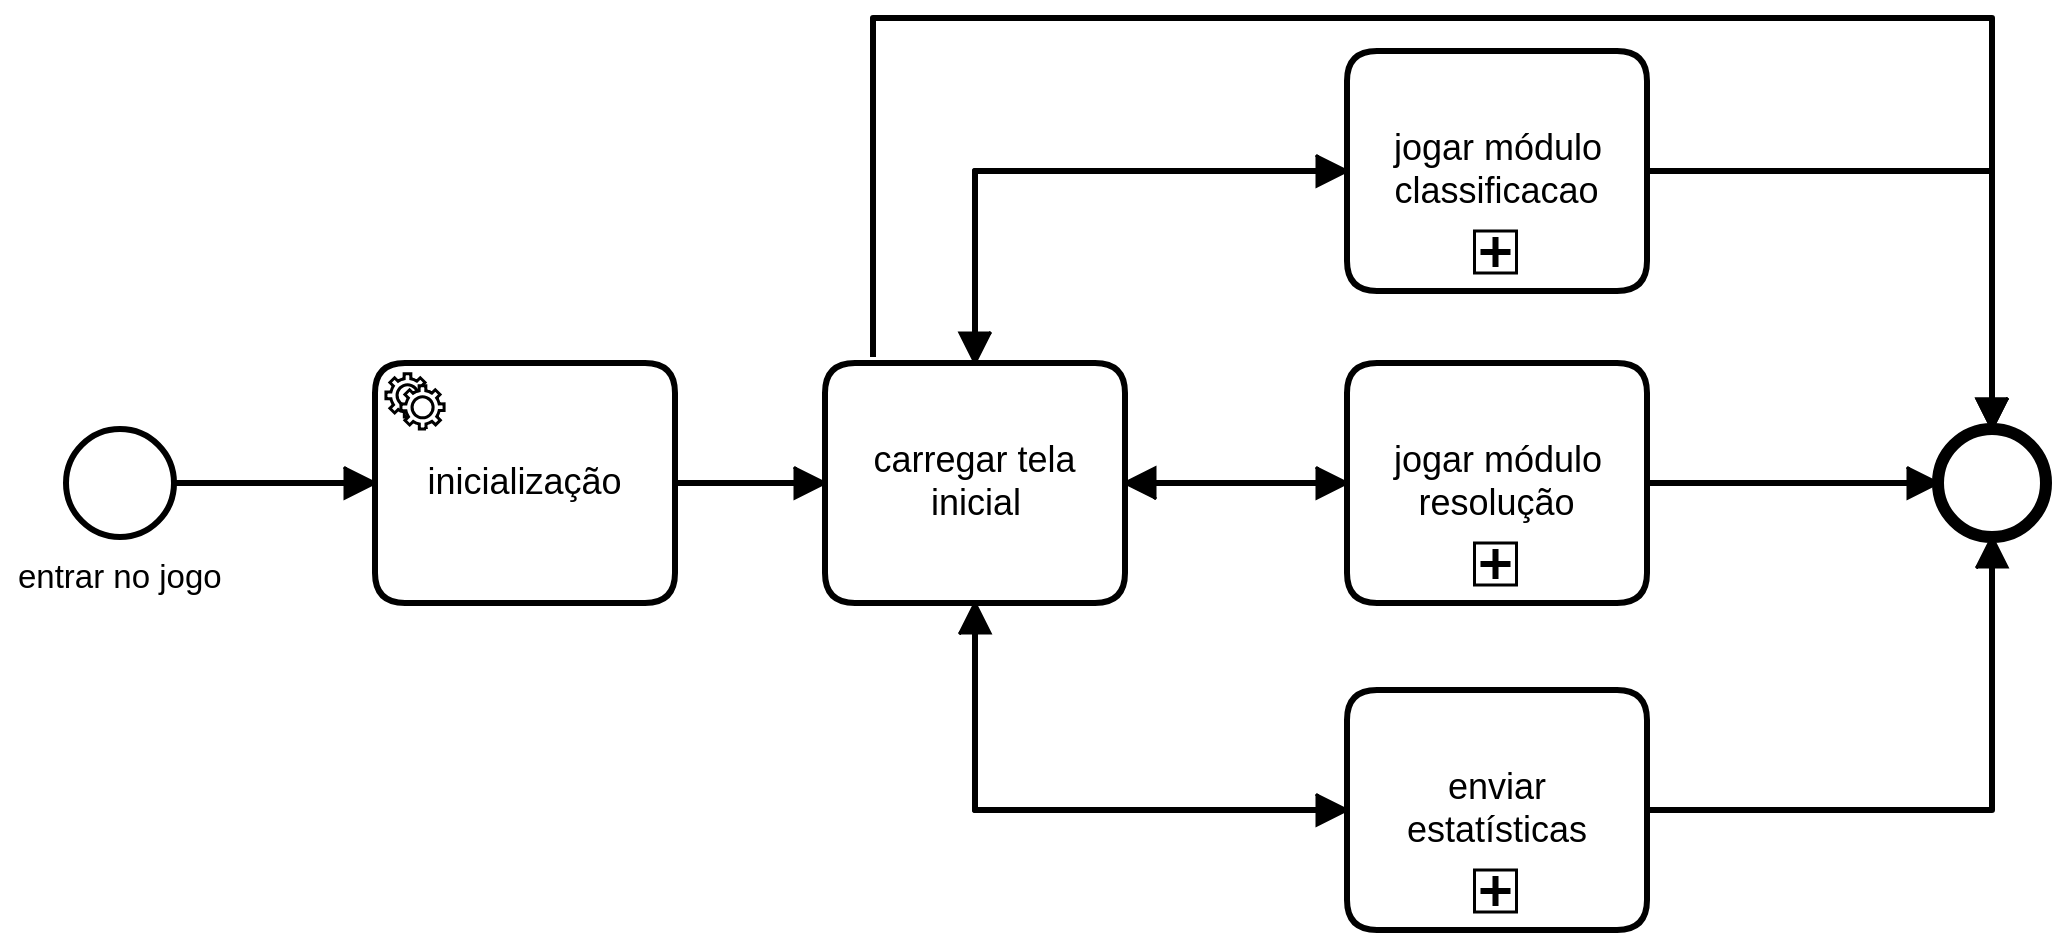
\includegraphics[scale=0.2]{figuras/processos/processo_geral.png}
\label{pg}
\\
\small{Fonte: do próprio autor}
\end{figure}

Na Figura \ref{pg} mostra-se que ao entrar no APP a primeira atividade é um script do sistema, assim que este termina é carregada a tela inicial que permite ao usuário jogar o módulo de classificação, jogar o módulo de resolução, enviar estatatísticas ou simplesmente sair do jogo sem fazer nada.

A primeira macro-atividade é a inicialização, indicada na Figura \ref{inic}.

\begin{figure}[H]
\centering
\caption{Processo de inicialização do jogo aprEnDO}
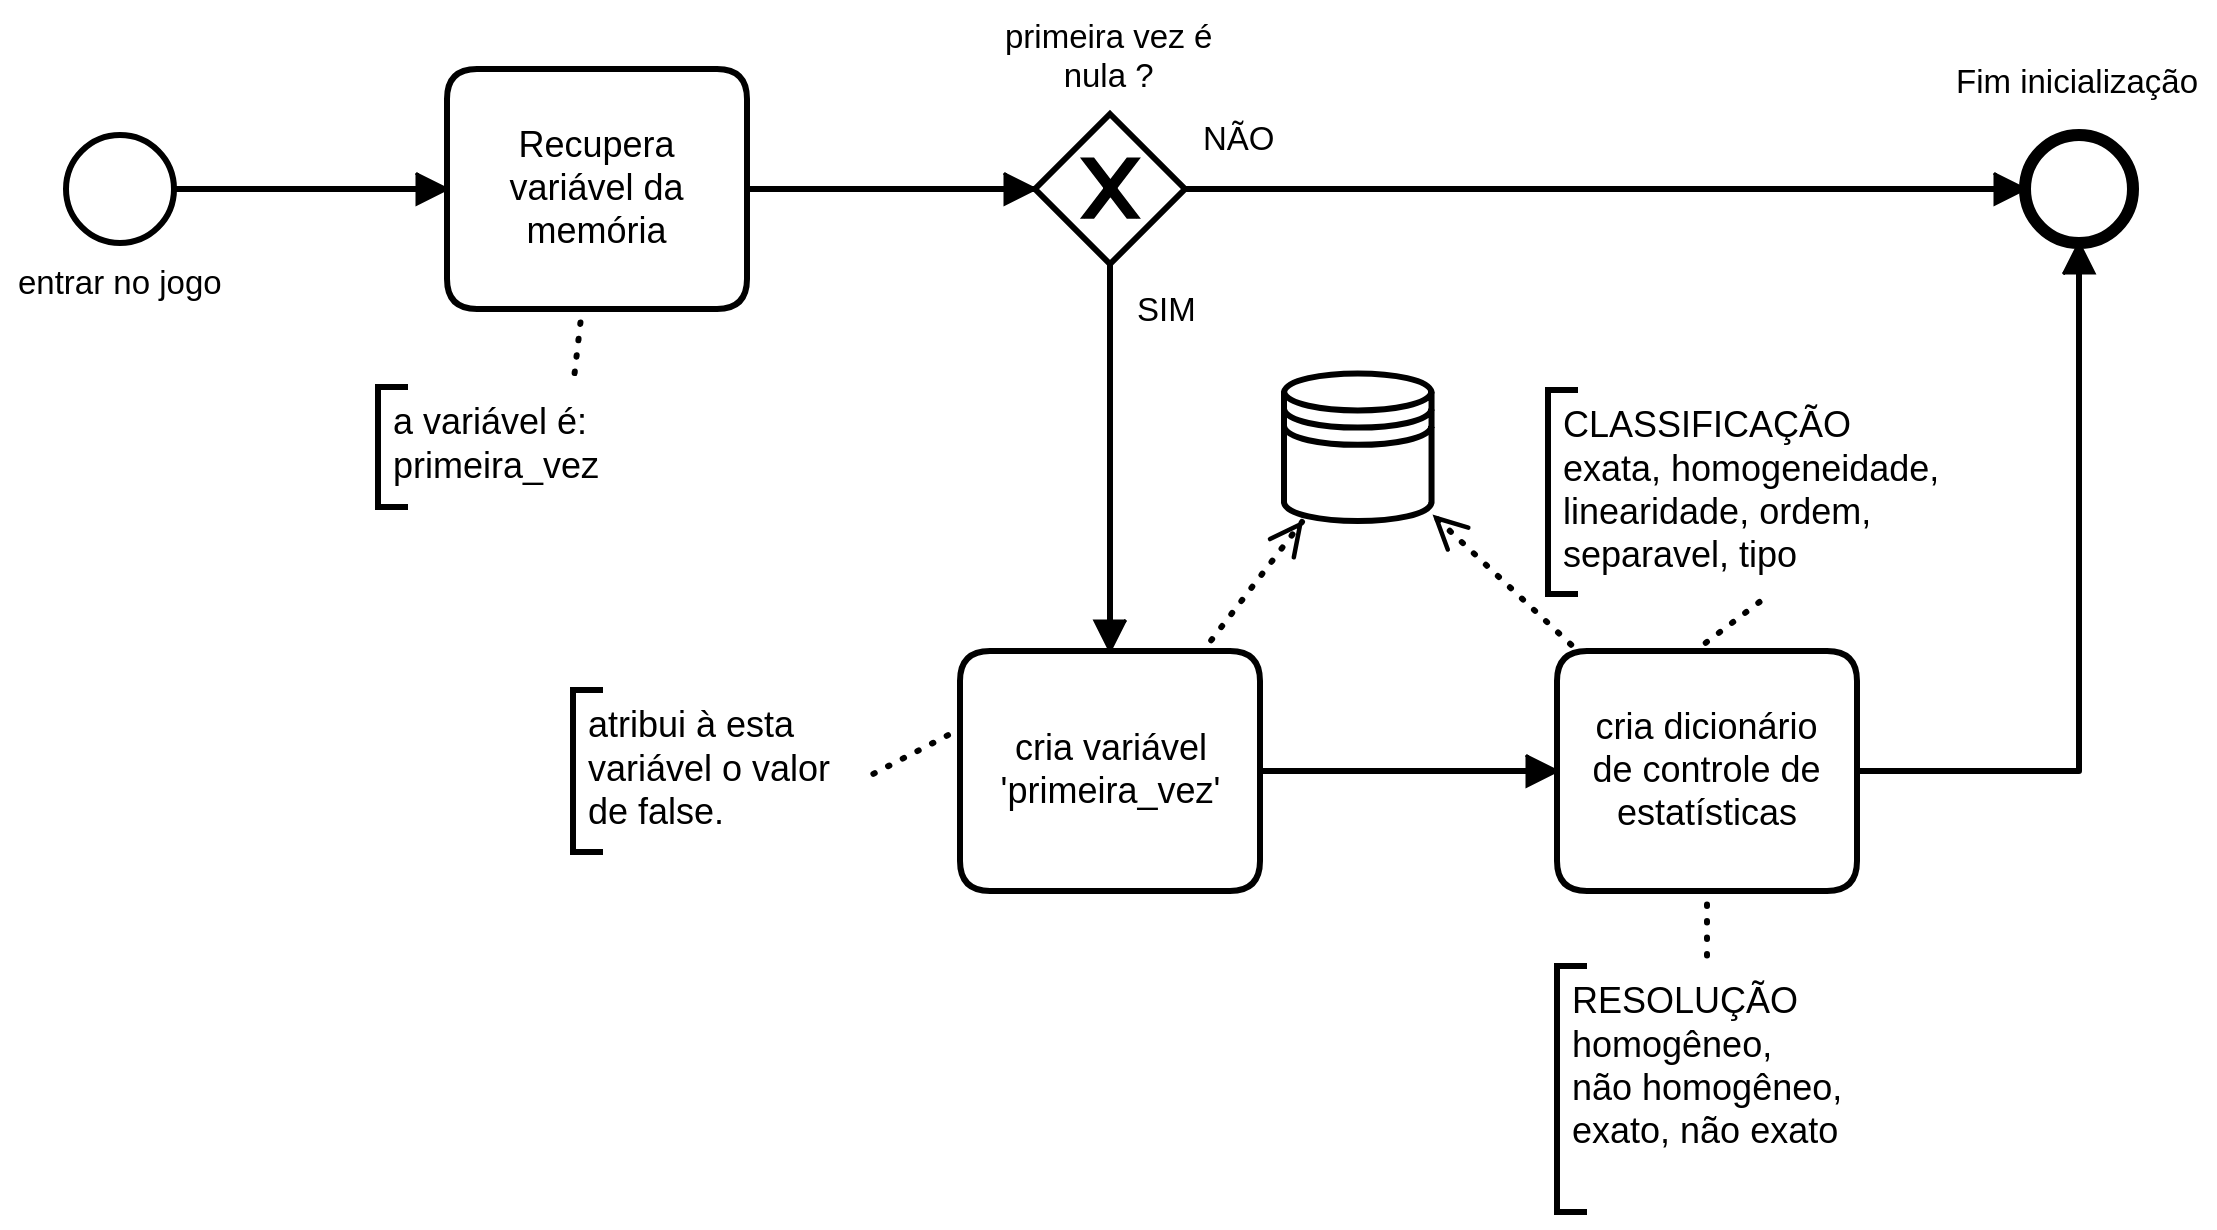
\includegraphics[scale=0.2]{figuras/processos/proccesso_inicializacao.png}
\label{inic}
\small{Fonte: do próprio autor}
\end{figure}

O processo \ref{inic} recupera a variável 'primeira\_vez' da memória, caso a variável exista e tenha o valor de 'falso' significa que o usuário já jogou outras vezes, então o processo termina. Caso seja realmente a primeira vez do usúário é necessário criar a variável 'primeira\_vez' para sinalizar que não é mais a primeira vez. Também é criado a estrutura de estatísticas para classificação e resolução e persistida no banco de dados do celular.

A segunda macro\-atividade é o processo de jogar o módulo de classificação, nele o usuário precisa escolher alguma fase de classificação. A Figura \ref{class_proc} mostra quais são as possíveis ações a serem tomadas pelo jogador.

\begin{figure}[H]
\centering
\caption{Processo de jogo de classificação}
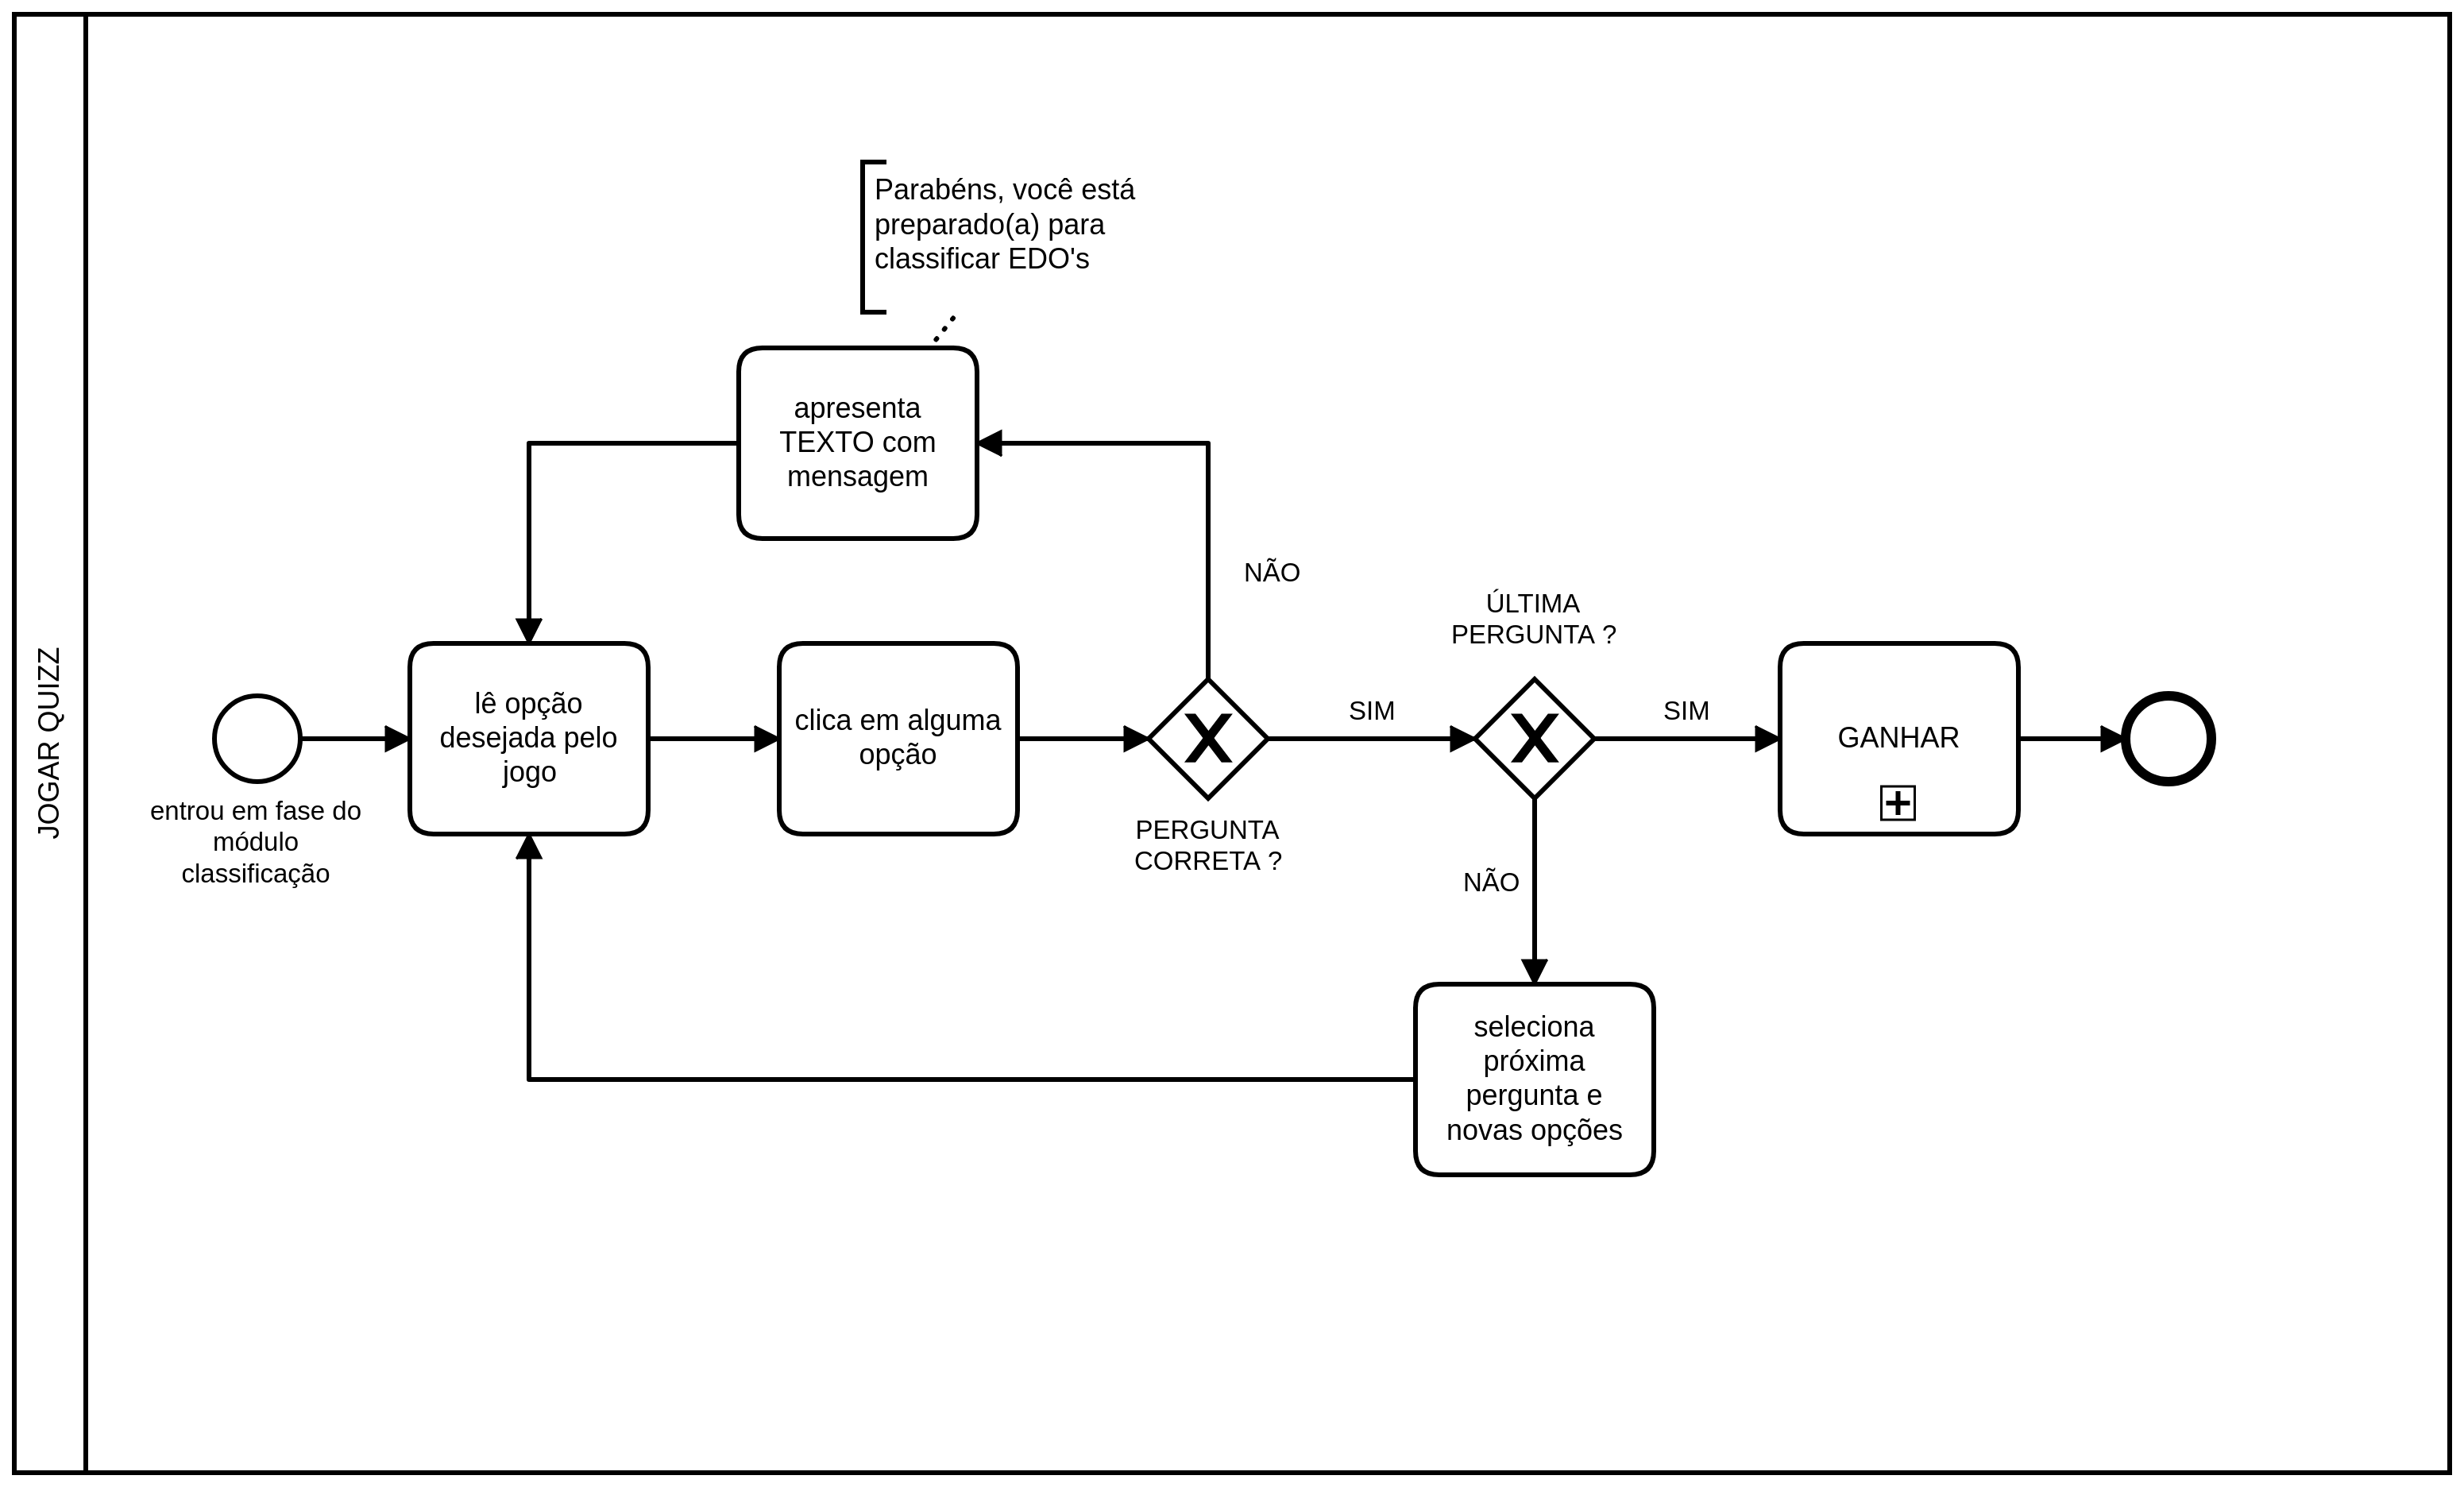
\includegraphics[scale=0.15]{figuras/processos/processo_classificacao.png}
\label{class_proc}
\small{Fonte: do próprio autor}
\end{figure}

Ambos os módulos \ref{class_proc} e \ref{res_proc} podem ativar o processo da Figura \ref{ganhar_proc} que consiste em armazenar as estatísticas de mais uma vitória nos dados do celular para que possam ser enviados ao servidor de coleta.


\begin{figure}[H]
\centering
\caption{Processo de ganhar uma fase}
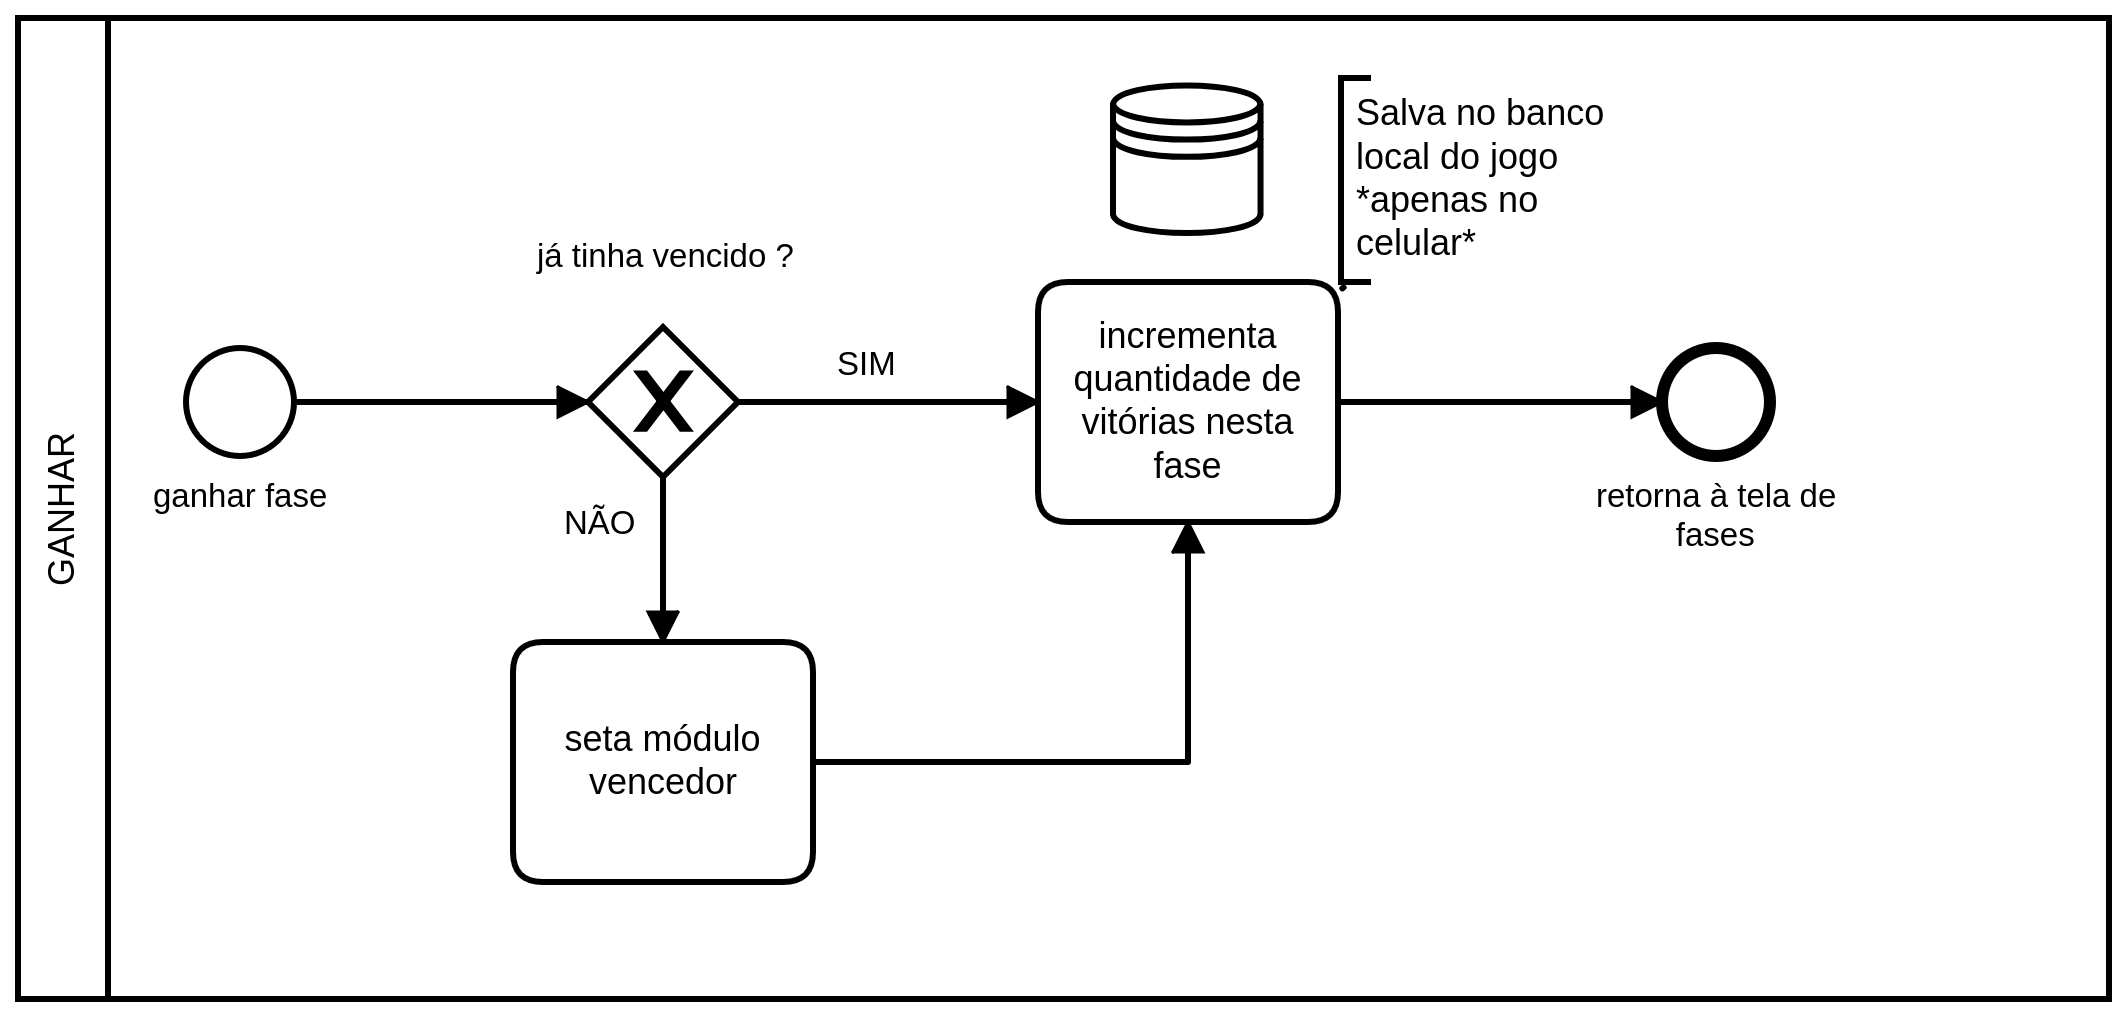
\includegraphics[scale=0.23]{figuras/processos/processo_ganhar.png}
\label{ganhar_proc}
\small{Fonte: do próprio autor}
\end{figure}


\begin{figure}[H]
\centering
\caption{Processo de jogo de resolução}
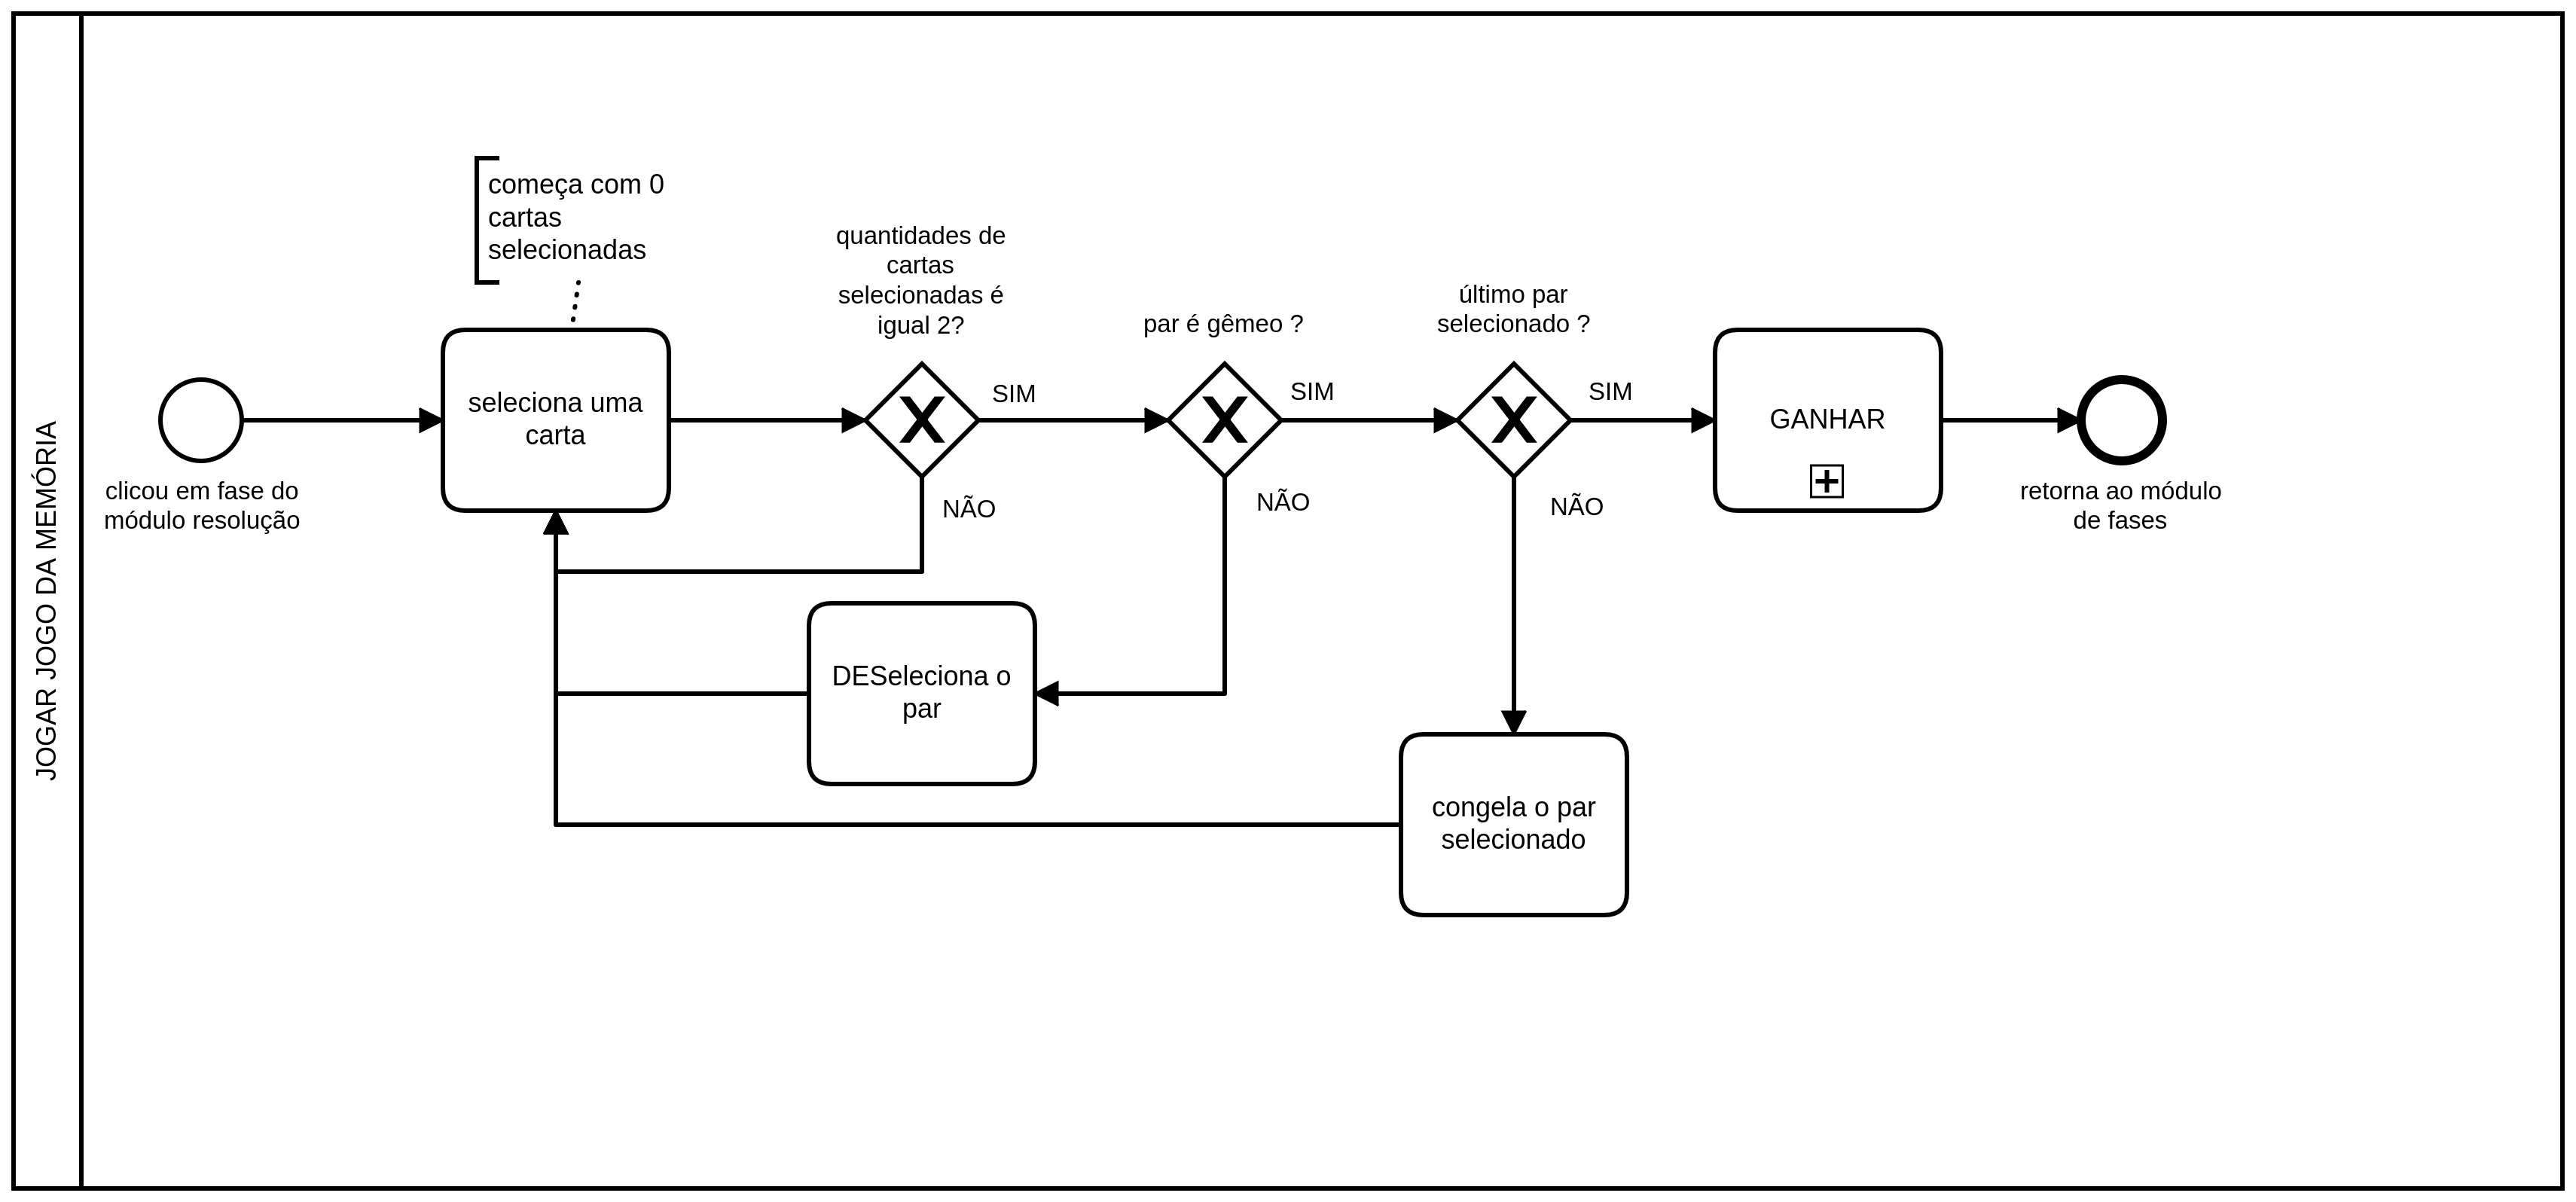
\includegraphics[width=\textwidth,height=\textheight,keepaspectratio]{figuras/processos/processo_resolucao.png}
\label{res_proc}
\small{Fonte: do próprio autor}
\end{figure}

A macro-atividade "GANHAR" presente nas Figuras \ref{class_proc} e \ref{res_proc} envolve o envio de estatísticas de jogo para um servidor de análise e coleta. O processo é detalhado na Figura \ref{envio_estatisticas}.

\begin{figure}[H]
\centering
\caption{Envio de estatísticas}
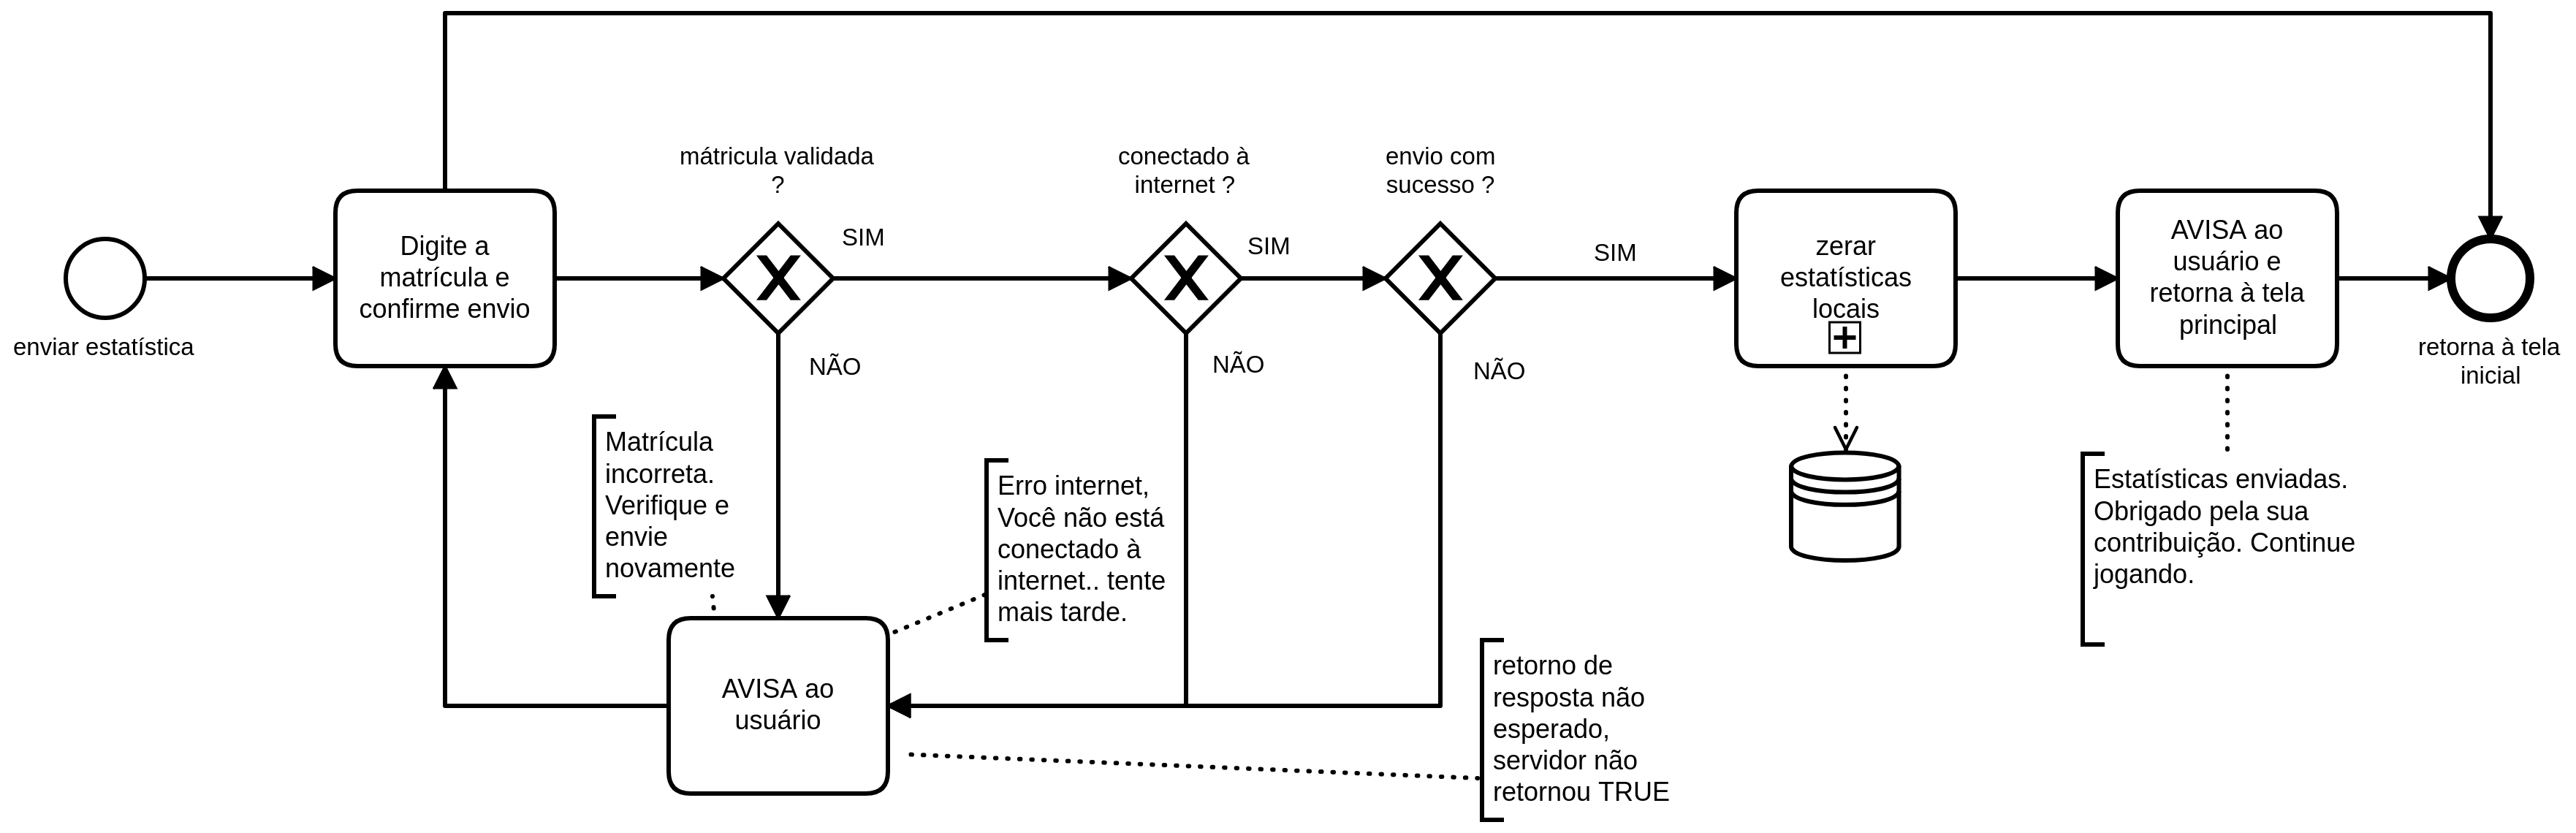
\includegraphics[width=\textwidth,height=\textheight,keepaspectratio]{figuras/processos/processo_enviar_estatisticas.png}
\label{envio_estatisticas}
\small{Fonte: do próprio autor}
\end{figure}

É necessário que o jogador digite sua matrícula corretamenta, pois esta será validada com a quantidade de 8 algarismos. Caso a matrícula seja validada e haja a conexão com a internet ocorrerá o envio dos dados, qualquer erro pelo caminho haverá o aviso específico ao jogador. Após a persistência dos dados no servidor, os dados locais são zerados para que não sejam redundantes no próximo envio. O processo de zerar estatísticas é apresentado na Figura \ref{zerar_estatisticas}. 

\begin{figure}[H]
\centering
\caption{Zerar estatísticas após envio}
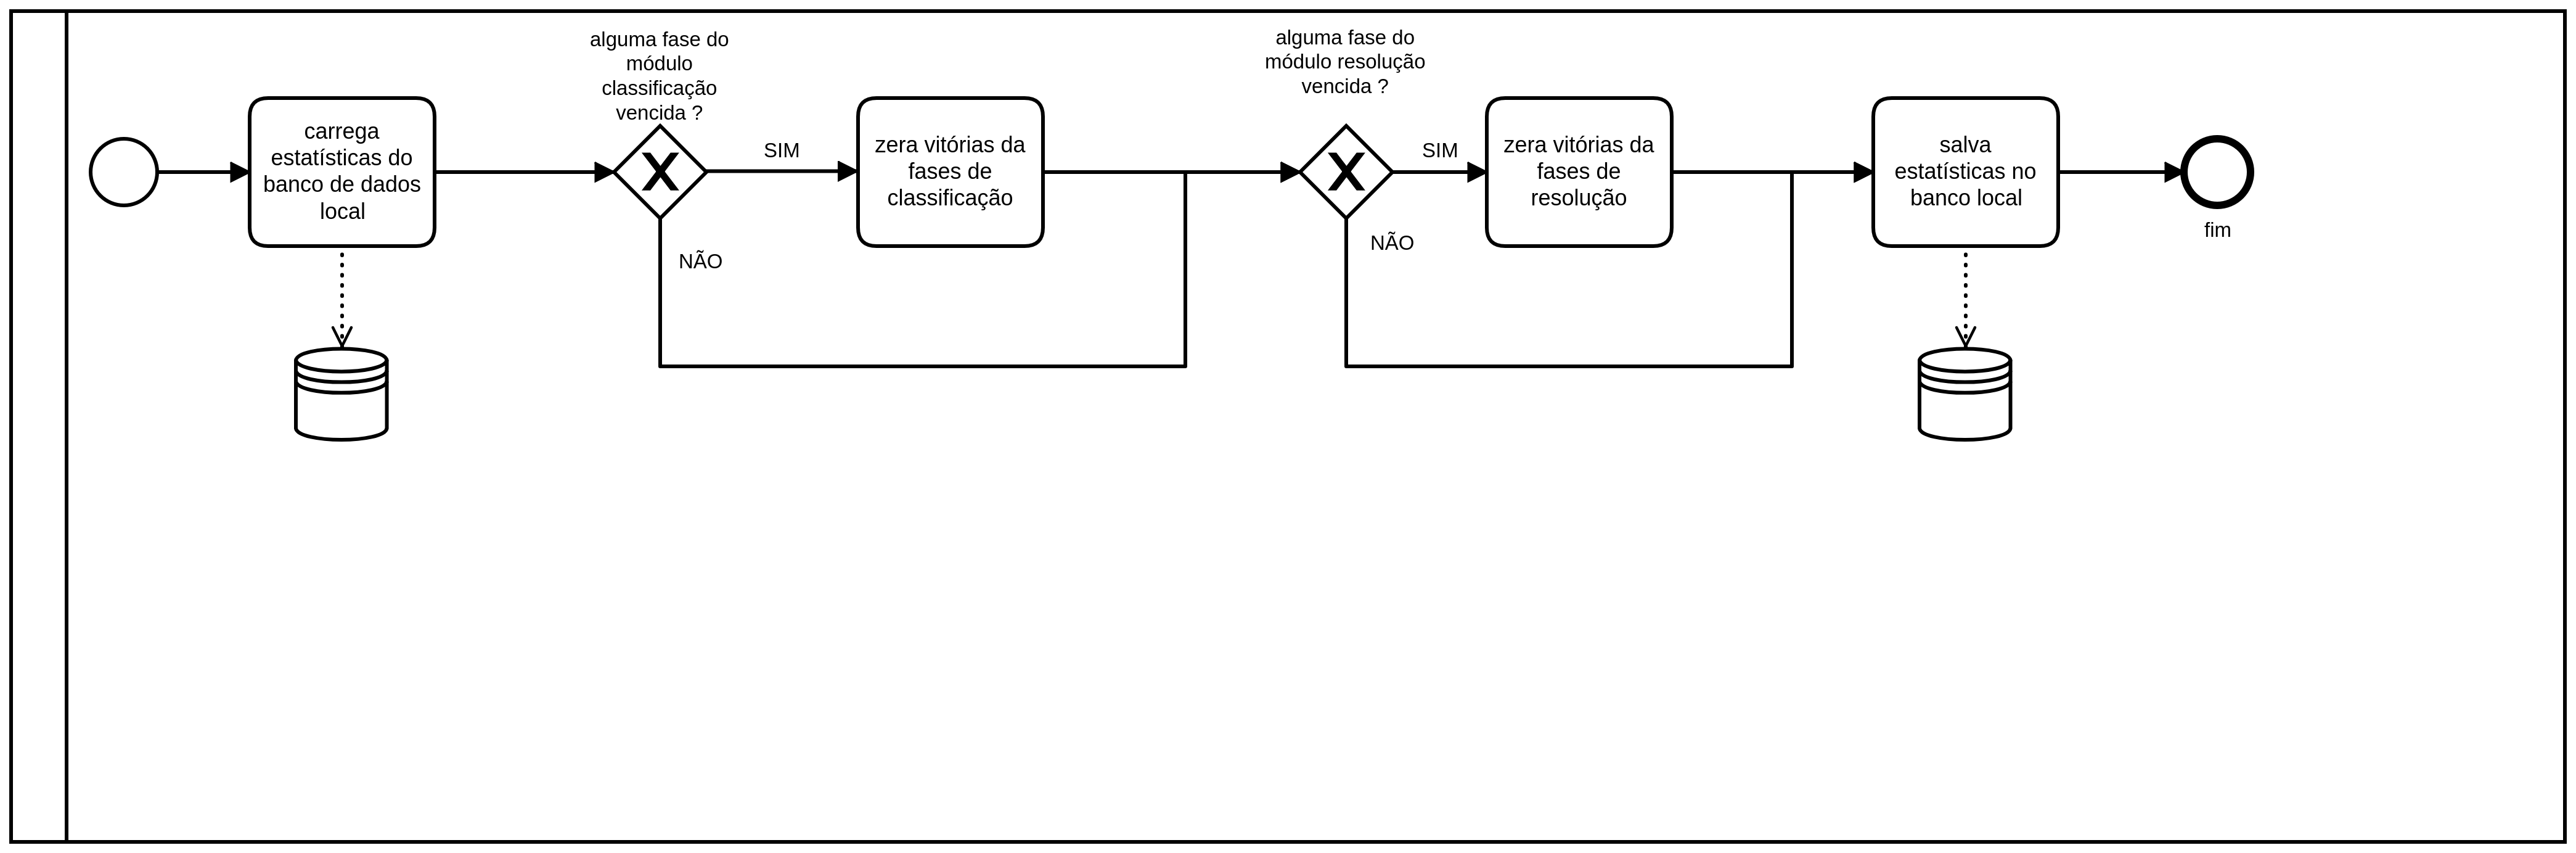
\includegraphics[width=\textwidth,height=\textheight,keepaspectratio]{figuras/processos/processo_zerar_estatisticas.png}
\label{zerar_estatisticas}
\small{Fonte: do próprio autor}
\end{figure}

Zerar estatísticas percorre as fases de classificação e resolução verificando qual fase já foi completada ao menos uma vez e trocando o valor atual para 0. Após o loop nos módulos os dados são persistidos na memória do celular.

Outro artefato de documentação desenvolvido foi o diagrama de classes. Este foi modelado de modo a facilitar o desenvolvimento e o entendimento da pasta src, pois deu uma guiada no que precisava ser feito e como as classes do jogo e os componentes se relacionam. 

\begin{figure}[H]
\centering
\caption{Diagrama de Classe do AprEnDO}
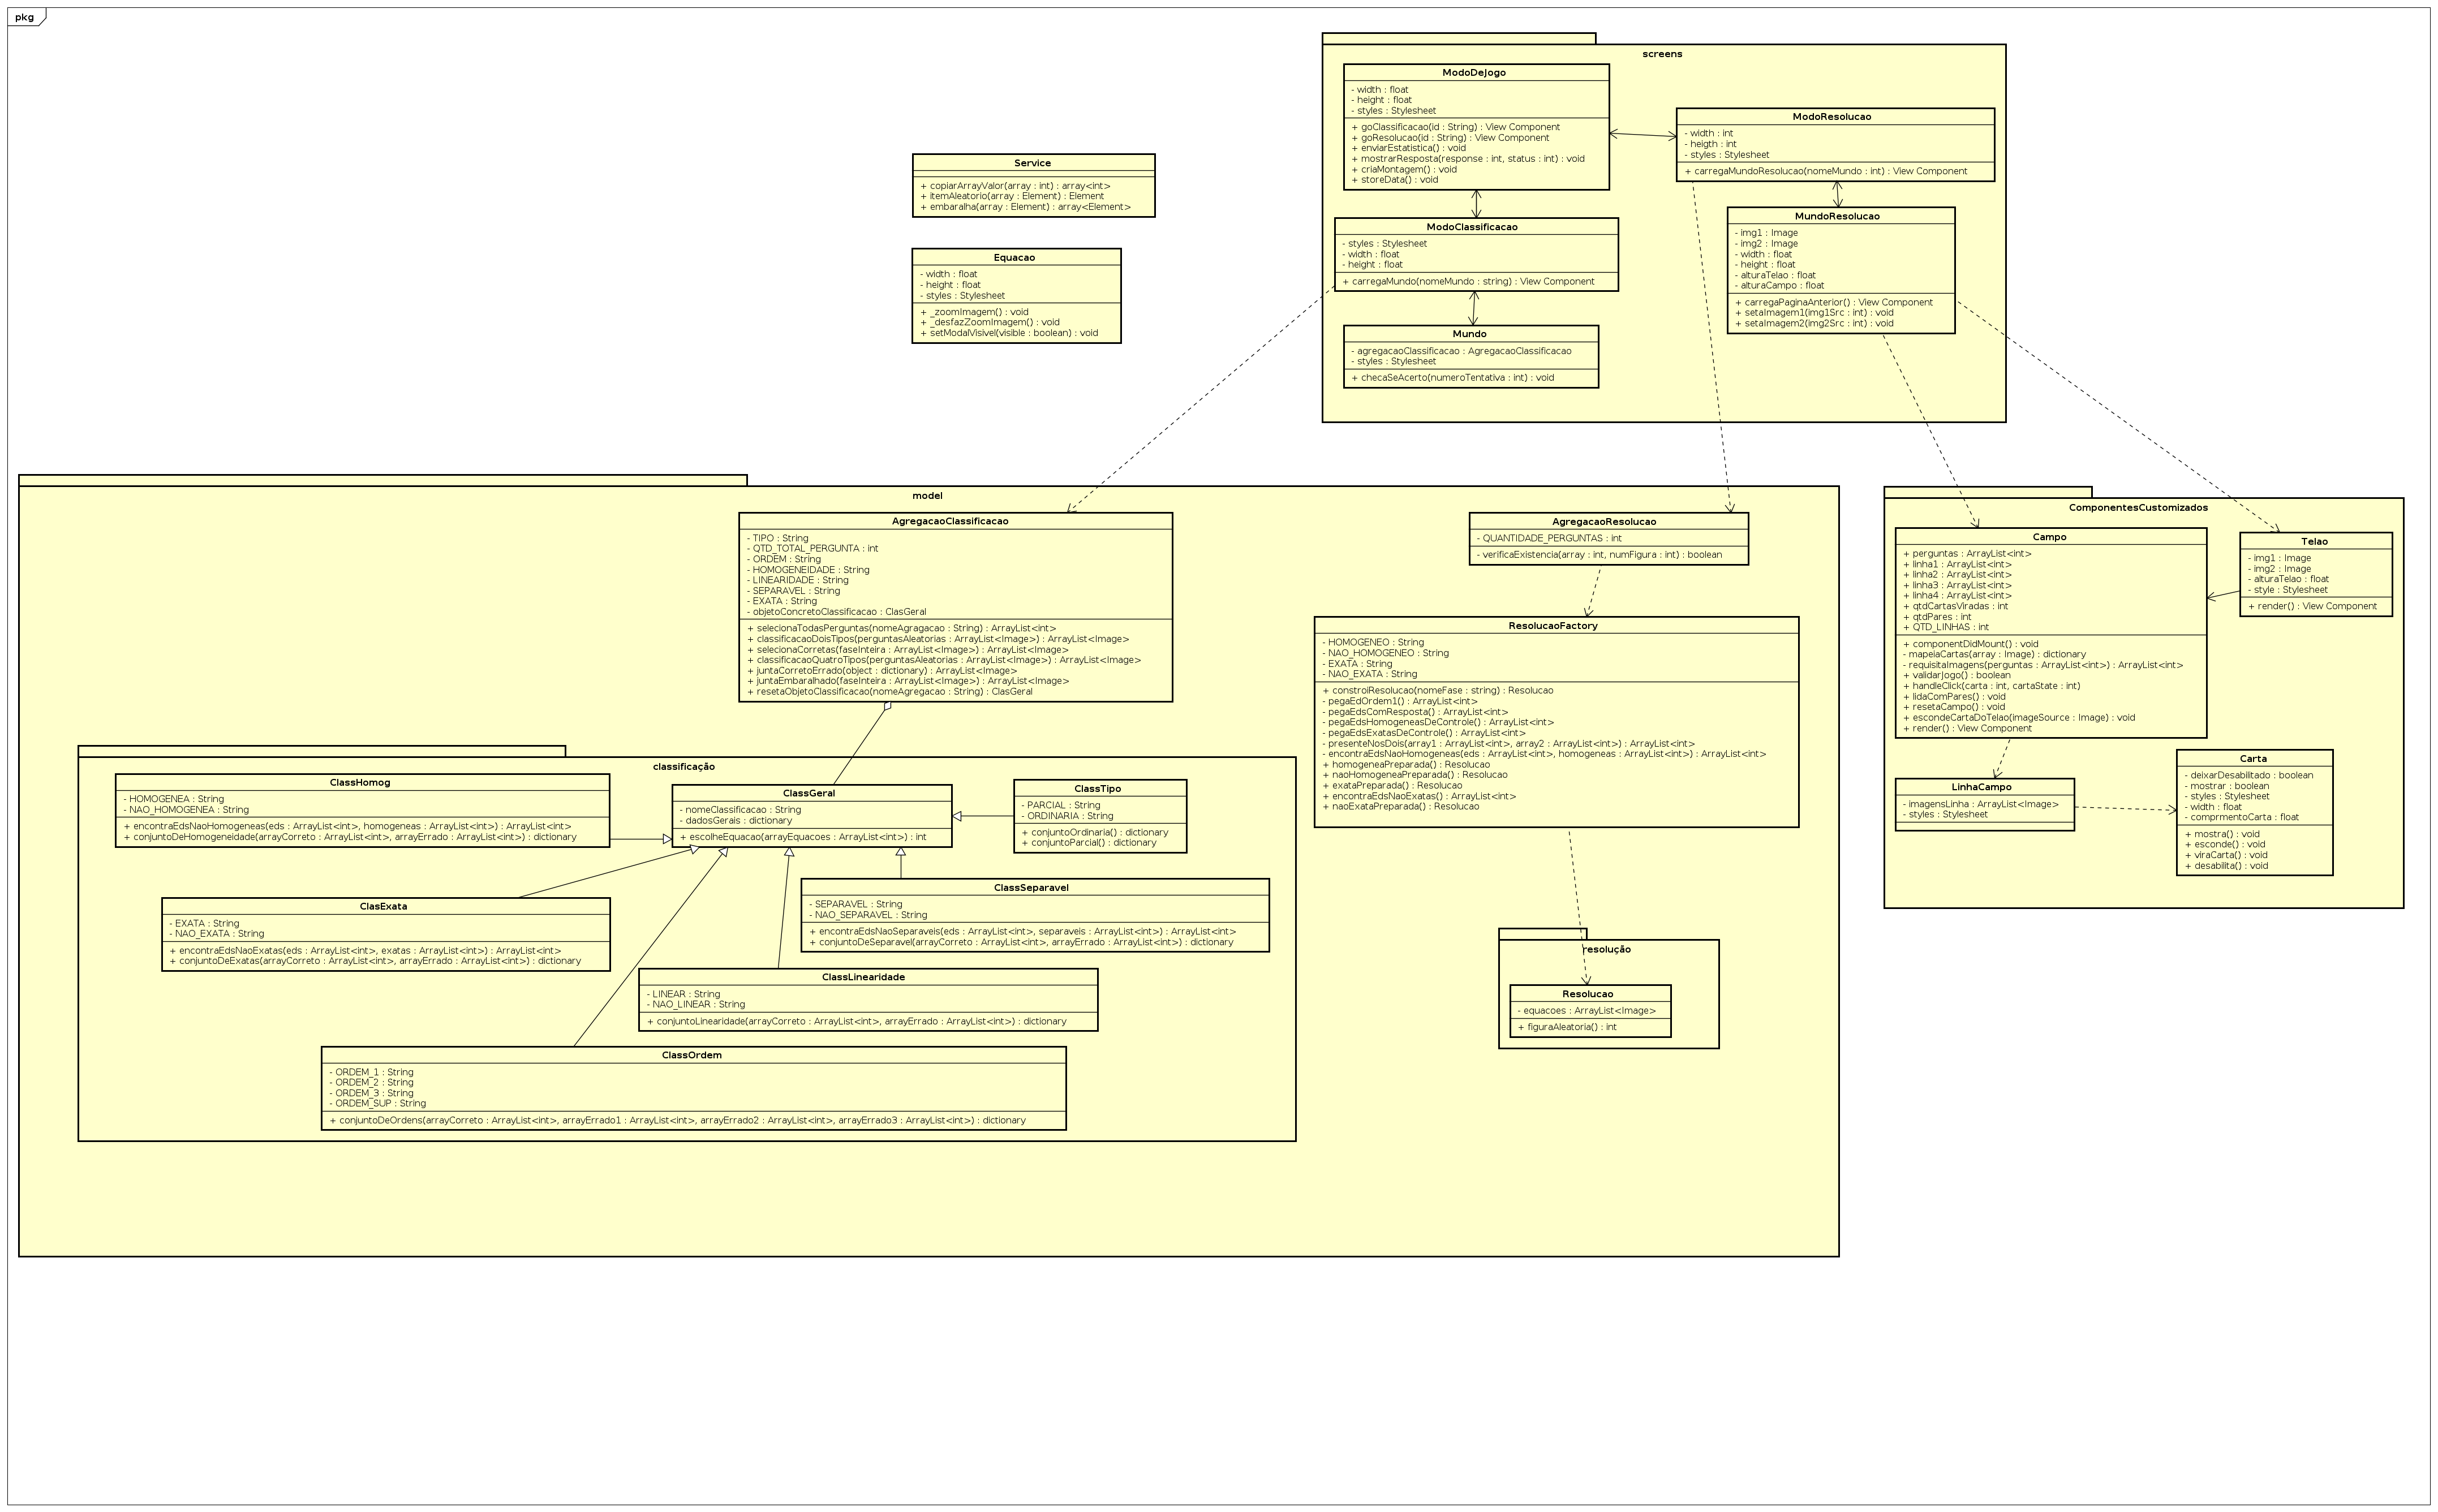
\includegraphics[width=\textwidth,height=\textheight,keepaspectratio]{figuras/DC_novo2.png}
\small{Fonte: do próprio autor}
\end{figure}

A pasta src apresenta o código fonte escrito em React (node.js).
A modelagem da aplicação é possível visualizar no diagrama de classe. Tem-se a pasta dos componentes customizados, a pasta model (que tem o modelo de perguntas e respostas e classes construtoras da agregação de perguntas e respostas para o jogo),  a pasta screens que contém as telas de jogo, sendo que algumas screens contém componentes que estão na pasta de componentes customizados. Tem o arquivo Service.js que realiza algumas tarefas auxiliares necessárias em partes misturadas do jogo, como por exemplo embaralhar um array (conjunto de dados homogêneos), realizar uma cópia de valores de um array e escolher um item aleatório.

\begin{comment}
VARIÁVEIS  

agregaçãoResolução
\label{agregaçãoResolução}

agregacaoClassificação
\label{agregacaoClassificação}

primeira\_vez
\label{primeira_vez}

mundo\_resolucao
\label{mundo_resolucao}

todasPerguntas
\label{todasPerguntas}

imgSrc
\label{imgSrc}
\end{comment}

A seguir uma explicação das funções desenvolvidas que estão na pasta SRC e suas subpastas.

\textbf{PASTA: SRC}
\begin{itemize}
\item ARQUIVO:Service
	\begin{itemize}
		\item copiarArrayValor: recebe um vetor como parâmetro e copia apenas os seus valores sem manter a referência. Para isso criar um vetor vazio, percorre o recebido e escreve seus valores no novo vetor que será retornado.

		\item itemAleatorio: recebe um vetor como parâmetro. Em caso de não pelo menos um elemento, nulo é retornado. Caso contrário com o apoio da biblioteca Math de matemática, um número flutuante entre 0 e 1 é escolhido e multiplicado pelo comprimento do vetor. O número é arredondado para baixo e então o item nesta posição do vetor é retornado.

		\item embaralha: recebe um vetor e aleatoriamente troca as posições dos valores

	\end{itemize}
\end{itemize}


\begin{itemize}
	\item ARQUIVO:Equacao

	\begin{itemize}

		\item \_zoomImagem: função ativada quando houver um longo clique em cima de algum exemplo de equação. Esta habilita o aparecimento de uma modal para mostrar equação ampliada.

		\item \_desfazZoomImagem: função ativada quando o dedo é tirado da tela após um longo clique em cima de algum exemplo de equação. Esta desabilita o aparecimento de uma modal que mostra equação ampliada.

		\item setModalVisivel: função chamada por \hyperref[_zoomImagem]{\_zoomImagem} e \hyperref[_desfazZoomImagem]{\_desfazZoomImagem} para habilitar ou desabilitar o aparacimento da modal com equação ampliada.
	
	\end{itemize}
	
\end{itemize}

\textbf{PASTA:SRC/screens}
\begin{itemize}
\item ARQUIVO:ModoDeJogo
	\begin{itemize}
	\item goClassificacao: a função goClassificacao utiliza a dependência Navigation e serve para redirecionar para a tela de classificação das equações diferenciais. Recebe como parâmetro um ID que é um identificador único do tipo string referente ao nome da screen que é para redirecionar.

	\item goResolucao: a função goResolucao utiliza a dependência Navigation importada no projeto que serve para redirecionar para a tela de resolução das equações diferenciais. Recebe como parâmetro um ID que é um identificador único do tipo string referente ao nome da screen que é para redirecionar.

	\item enviarEstatísticas: a função enviarEstatisticas funciona de modo assíncrono e utiliza da dependência netInfo para checar seu dispositivo está conectado à internet. Caso o dispositivo não esteja, um alerta avisando ao usuário que não está conectado à Internet é acionado e retorna a página inicial da aplicação, caso haja conexão com a internet é checado se a matrícula digitada pelo usuário não é nula e ao remover os caracteres de barra de espaço verifica-se que não está vazio e que contém 8 dígitos. Em caso de matrícula inserida corretamente é acionado um loader enquanto as estatísticas locais do celular são capturados e formatadas para então realizar uma requisição ao servidor do Heroku na rota ‘/estatísticas’. O conteúdo JSON é formatado para string e então enviado. Após o processamento no servidor uma resposta é retornada para o aplicativo e a função enviarEstatisticas chama a função mostraResposta que tratará de mostrar a resposta adequada a depender do status de retorno do Servidor. Em caso de alguma exceção ocorrer durante todo o processamento um alerta é mostrado ao usuário indicando que houve erro com o servidor e pedindo para retornar mais tarde. O loader é desabilitado e novamente retorna-se a tela inicial da aplicação.

	\item mostraResposta: a função mostraResposta é acionada pela função enviarEstatisticas e também assíncrona. Recebe como parâmetro a resposta do Servidor e o código de status. Caso a resposta tenha sucesso NÃO OKAY é mostrado um alerta para o usuário informando retorno não esperado e retorna-se à tela inicial. Em caso de resposta sucesso OKAY é carregado da memória local as estatísticas atuais e um loop percorre todas as fases do modo de classificação e de resolução zerando a quantidade de vezes que o jogador terminou de jogar, para que no próximo envio seja enviado apenas as variações entre o último envio e o atual. Após as estatísticas estarem zeradas, sstas são salvas na memória do celular e um alerta de estatísticas enviadas com sucesso é apresentado ao usuário, só então retorna-se a tela inicial.

	\item criaMontagem: a função é acionada apenas na primeira vez o que o jogador acessa o jogo para então criar o template das estatísticas de classificação e resolução e todas as suas fases e assim é salvo na memória do celular. O tipo de dado das estatísticas é um Json.

	\item storeData: a função storeData é acionada toda vez que um jogador entra no jogo. É tentado recuperar da memória uma variável chamada \ref{primeira_vez}, caso esta variável seja nula significa que é a primeira vez do usuário no jogo, esta variável é então criada e salva na memória com valor falso para nas outras vezes não cair neste caso, chama-se a função \ref{criaMontagem} para gerar o template das estatísticas. Caso a variável \ref{primeira_vez} já exista e retorne o valor de falso, significa que não é a primeira vez do usuário no jogo e nada acontece.

	\end{itemize}
\end{itemize}

\begin{itemize}
\item ARQUIVO:ModoClassificacao
	\begin{itemize}
	\item carregaMundo: função assíncrona que tem como parâmetro o nome de mundo que será criado para ser repassado ao objeto agregação classificação. Este objeto serve para a função na hora de chamar a nova tela de mundo passando as propriedades: vetor de perguntas aleatórias criadas, vetor do número das imagens corretas, vetor das fases embaralhadas, o total de questões e o nome do mundo.
	\end{itemize}
\end{itemize}

\begin{itemize}
\item ARQUIVO:ModoResolucao
	\begin{itemize}	
	\item carregaMundoResolucao: função assíncrona que recebe como parâmetro o nome do mundo para criar objeto agregaçãoResolução e passar para próxima \textit{screen} chamada \ref{mundo_resolução} junto com a propriedade \ref{todasPerguntas} que é um vetor provido pelo objeto agregaçãoResolução
	\end{itemize}	
\end{itemize}	

\begin{itemize}
\item ARQUIVO:Mundo
	\begin{itemize}
	\item checaSeAcerto: função assíncrona é ativada assim que alguma opção de classificação é clickada. Recebe como parâmetro o número da tentativa da rodada, que varia de 1 a 4. Caso o número da tentativa clicada seja igual ao da pergunta correta o número da perguntaAtual é incrementado e o número da quantidade de perguntasCorretas também é incrementado apenas em caso de não ser a última pergunta. Em caso de ser a última pergunta e tentativa estiver correta as estatísticas são atualizadas com o incremento de uma vitória na fase jogada do módulo de classificação. Ao vencer a fase um alerta de parabenização é mostrado e abre-se uma janela que ao ser confirmada retorna à tela de classificação. No caso de tentativa incorreta é mostrado um alerta de tente novamente e retorna-se à questão pendente. 
	\end{itemize}
\end{itemize}

\begin{itemize}
\item ARQUIVO:MundoResolucao
	\begin{itemize}
	\item carregaPaginaAnterior: utiliza a dependência Navigation e apenas fecha a página atual que a página anterior já está na pilha e passa então a ser a atual.
	\end{itemize}
\end{itemize}


\textbf{PASTA:SRC/model}
\begin{itemize}
	\item ARQUIVO:AgregacaoClassificacao
	\begin{itemize}
		\item selecionaTodasPerguntas: este método recebe o parâmetro do nome da fase de classificação e retorna um array com a escolha aleatória de vinte perguntas da fase que será jogada.
		\item classificacaoDoisTipos: esta função serve para todas as fases de classificação que tem apenas duas perguntas (tipo, homogeneidade, linearidade, separável e exata). Não serve apenas para "ordem". A função recebe o array de vinte perguntas aleatórias e para cada pergunta monta um dicionário com uma equação correta e três equações erradas. Esse conjunto é adicionado a um array. É retornado o array de dicionário com vinte conjuntos.
		\item selecionaCorretas: Recebe como parâmetro o array de dicionários com os vinte conjuntos. Monta-se um array com o número das vinte equações corretas e este array é retornado.  
		\item classificacaoQuatroTipos: esta função serve para todas as fases de classificação que tem apenas quatro perguntas, que no caso é apenas para "ordem". A função recebe o array de vinte perguntas aleatórias e para cada pergunta monta um dicionário com uma equação correta e três equações erradas. Esse conjunto é adicionado a um array. É retornado o array de dicionário com vinte conjuntos.
		\item juntaCorretoErrado: recebe um dicionário como parâmetro que contém as chaves "correto" e "errado". O correto tem apenas um número de equação e o errado tem três números de equação. Todos os número de equação do dicionário são adicionados a um único array e este é retornado. 
		\item  juntaEmbaralhado: recebe como parâmetro o array de dicionários e embaralha as quatro questôes de cada fase, de modo que a equação correta não fique sempre na mesma posição. É retornado o array com todas as equações da fase embaralhado.
		\item resetaObjetoClassificacao: recebe como parâmetro um nome da fase e retorna um objeto especializado do norme da fase. Pode ser tipo, ordem, homogeneo, linearidade, separável ou exata.
	\end{itemize}
\end{itemize}

\begin{itemize}
	\item ARQUIVO:AgregacaoResolucao
	\begin{itemize}
		\item verificaExistencia: recebe como parâmetro um array com número de figuras e o número de uma figura. Retorna verdadeiro caso o número da equação esteja contido no array e retorna falso caso o número da equação não esteja no array.
	\end{itemize}
\end{itemize}

\begin{itemize}
	\item ARQUIVO:ResolucaoFactory
	\begin{itemize}
		\item constroiResolucao: este método recebe como parâmetro o nome da fase para retornar o objeto com as equações possíveis do arquivo de controle 
		\item pegaEdOrdem1: 
		\item pegaEdsComResposta: 
		\item pegaEdsHomogeneasDeControle:
		\item pegaEdsExatasDeControle:
		\item presenteNosDois: 
		\item encontraEdsNaoHomogeneas:
		\item homogeneaPreparada:
		\item naoHomogeneaPreparada:
		\item exataPreparada:
		\item encontraEdsNaoExatas: 
		\item naoExataPreparada: 
	\end{itemize}
\end{itemize}

\textbf{PASTA:SRC/model/classificação}

\textbf{PASTA:SRC/model/resolução}


\textbf{PASTA:SRC/ComponentesCustomizados}
\begin{itemize}
\item ARQUIVO:Campo
	\begin{itemize}
	\item mapeiaCartas: recebe o array retornado da requisitaImagens o qual inicia-se com uma pergunta e sucessivamente sua solução. Um loop é feito no array para criar um dicionário com chaves as perguntas e valor as respostas. Por isso o loop é iterado apenas nas perguntas, que são as posições pares. Ao final da iteração e população do dicionário, o mesmo é retornado.
	
	\item requisitaImagens: recebe um array com o número das figuras aleatórias sorteadas para esta partida e faz o import através da função require procurando no arquivo index das perguntas e das respostas. O retorno é um array com vinte figuras, sendo dez perguntas e dez soluções das perguntas. OBS: o array de retorno é ordenado com uma pergunta e a sua solução sucessivamente.

	\item validarJogo: é chamada sempre que duas cartas estão viradas para cima. A função serve para decidir se duas cartas formam um par. A verificação ocorre comparando com o array de cartas mapeado chave e valor. O procedimento checa se a primeira carta virada é chave ou valor. Se for chave, então compara a segunda carta com o valor, se for valor, procura-se então a chave para comparar com a segunda carta para assim confirmar se a dupla forma um par gêmeo ou não. Em caso de ser um par, pela regra do jogo é decrementado uma unidade dos pares restantes, se for o último par já acontece a atualização das estatísticas de qual fase do módulo resolução foi vencido e a parabenização ao usuário com retorno para a tela de escolha de fase. Se não for o último par, a função apenas retorna informando se as cartas atuais formam um par ou não.

	\item handleClick: é acionada quando ocorre o click em qualquer carta enviando a informação se a carta é para ser virada ou escondida (true ou false). Se for um click para mostrar a carta, então a variável quantidadeDeCartasViradas é incrementado em 1. 
	OBS: Se esta for a única carta virada então na posição reservada para a imagem 1 será renderizada a equação da carta
	OBS1: Se for a segunda carta virada, a carta será desenhada no espaço reservado para a imagem 2 e será aplicado o procedimento do jogo da memória para validar se as 2 cartas foram um par. 

Se for um click para não mostrar a carta é acionada a função para esconder a carta do telão (espaço reservado para renderização das equações), e se o valor da variável não cair em nenhum dos casos previstos um novo erro é lançado.

	\item lidaComPares: é chamada pelo handleClick deste mesmo arquivo. Recebe como parâmetro um booleano que representa se as duas cartas viradas para cima formam um par ou não. Em caso de serem um par, as cartas tem a função de click desabilitadas, e são travadas viradas pra cima com a imagem da equação sendo mostrada. Em caso de não serem um par as duas são viradas para o lado inverso escondendo o seu conteúdo. 

	\item resetaCampo: esta função limpa as 2 equações renderizadas no telão, altera o estado de quantidadeDeCartasViradas para 0 e limpa o vetor de 2 posições que armazena as cartas viradas no momento.

	\item escondeCartaDoTelao: recebe como parâmetro a imgSrc da imagem a ser escondida. Para isso também é necessário decrementar a quantidade de cartas viradas em uma unidade e então checar qual das duas cartas do telão que tem a imgSrc igual ao que foi passado para esta função, para então poder setá-lo como nulo. 

	\end{itemize}
\end{itemize}

\begin{itemize}
\item ARQUIVO:Telao
\end{itemize}	


\begin{itemize}
\item ARQUIVO:LinhaCampo
\end{itemize}

	encaminha a função handle para cada carta do campo assim como o conteúdo da carta também, ou seja, a sua imagem, seja uma carta de pergunta, ou de resposta.
 
\begin{itemize}
\item ARQUIVO:Carta
	\begin{itemize}
	\item mostra: alterna o estado da variável mostrar e troca o valor da animação de 0 graus para 180 graus, realizando o efeito de virar a carta.

	\item esconde: alterna o estado da variável mostrar e troca o valor da animação de 180 graus para 0 graus, realizando o efeito de virar a carta e mostrar o fundo.

	\item viraCarta: checa o estado da variável mostrar para decidir se chama a função mostra ou esconde e chama a função handle que lida com as regras do jogo da memória.

	\item desabilita: troca o estado da variável deixarDesabilitado, a qual é chamada apenas quanto um par de cartas gêmeas é encontrado. Desse modo impede que a carta seja rotacionada desse momento para frente, deixando-a sempre virada com a parte do conteúdo para cima, porém desabilitada para cliques.

	\end{itemize}
\end{itemize}
